% ===Lesson 9: Cross-referencing
\documentclass{article}
\usepackage[T1]{fontenc}
\usepackage[margin=1in]{geometry}
\usepackage{graphicx}
\usepackage{array}
\usepackage[hidelinks]{hyperref}
\usepackage{verbatim}
\usepackage{xcolor}
\usepackage{soul}

\begin{document}
\hl{This lesson shows how to refer to numbered elements in a document, like figures, tables and sections.}

\section{The \texttt{label} and \texttt{ref} mechanism}
To have LaTeX remember a spot in your document you have to \textbf{label} it, and then in other places, you \textbf{refer} to it.

\begin{verbatim}
\begin{document}
Hey world!

This is a first document.

\section{Title of the first section}

Text of material for the first section.


\subsection{Subsection of the first section}
\label{subsec:labelone}

Text of material for the first subsection.
\begin{equation}
  e^{i\pi}+1 = 0
\label{eq:labeltwo}
\end{equation}

In subsection~\ref{subsec:labelone} is equation~\ref{eq:labeltwo}.
\end{document}
\end{verbatim}

The \verb|subsec:| and \verb|eq:| aren’t used by LaTeX; rather, it just keeps track of what it has most recently processed. But when you are writing these help you remember what the label is about.

Notice the tilde \verb|~| characters before the references. You don’t want a line break between subsection and its number, or between equation and its number. Putting in a tilde means LaTeX won’t break the line there.

\section{Where to put \texttt{label}}
The \verb|\label| command always refers to the previous numbered entity: a section, an equation, a float, etc. That means that \verb|\label| always has to come after the thing you want to refer to. In particular, when you create floats, the \verb|\label| has to come after (or better, in), the \verb|\caption| command, but within the float environment.

\section{Exercises}
\label{sec:exercies}
\paragraph{Ex1} Try adding new numbered parts (sections, subsections, enumerated lists) to the test document and finding out how many runs are needed to make \verb|\label| commands work.

It took me 1 time to successfully refer to the section \ref{sec:exercies}.

\paragraph{Ex2} Add some floats and see what happens when you put \verb|\label| before the \verb|\caption| instead of after; can you predict the result?

\begin{figure}[ht]
    \centering
    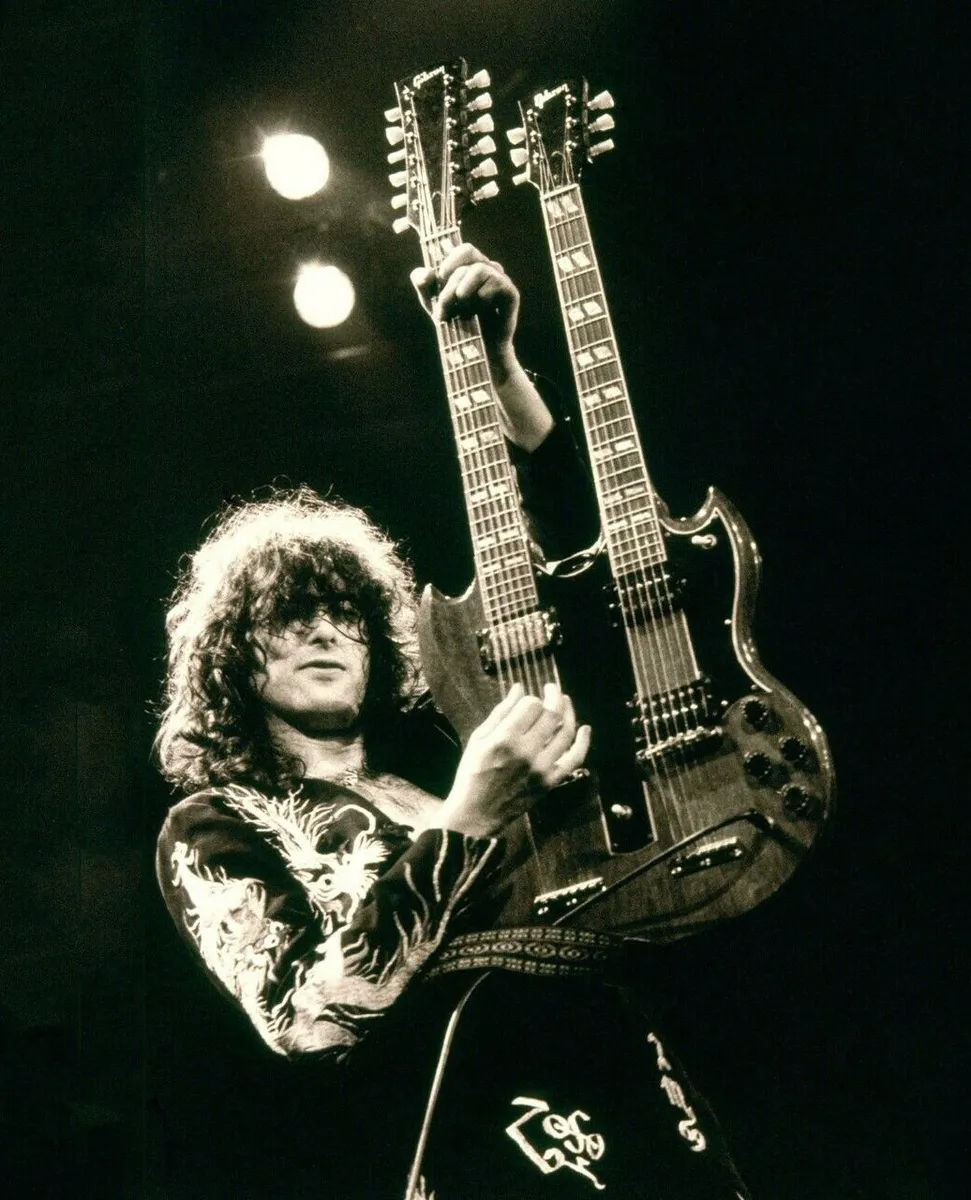
\includegraphics[width=5cm]{image/jimmy page.png}
    \caption{Jimmy Page}
    \label{fig:jimmy-page}
\end{figure}

Figure \ref{fig:jimmy-page} is an image of Jimmy Page.

\textbf{Answer:} LaTeX uses \verb|\caption| to set the number of the figure or table, and \verb|\label| picks up this number. When you place \verb|\label| after \verb|\caption|, it correctly references that figure or table. However, if you place \verb|\label| before \verb|\caption|, the \verb|\label| might refer to the most recently defined figure or table number (or none at all if it's the first instance).

\paragraph{Ex3} What happens if you put a \verb|\label| for an equation after the \verb|\end{equation}|?

\begin{equation}
    S = v \times t
    \label{eq:distance}
\end{equation}

Equation \ref{eq:distance} is the formula for computing the distance based on time and velocity.

\textbf{Answer:} Reference doesn't work if \verb|\label| is outside the environment. No explanation.
\end{document}
% End Lesson 9 (Nov 4 2024)===